\documentclass{article}

\usepackage{latexsym}
\usepackage{amsmath}
\usepackage{amssymb}
\usepackage{graphicx}
\usepackage{amsthm}
\usepackage{hyperref}

\newcommand*{\thead}[1]{\multicolumn{1}{|c|}{\bfseries #1}}

\newtheorem{theorem}{Theorem}
\newtheorem{question}{Question}

\begin{document}

\title{Euclid's Algorithm and B\'ezout's Identity}
\author{Dave Neary}

\maketitle

\section{Introduction}

When working with large numbers, we will often want to calculate their greatest common divisor.
In particular, it is often important to know if two numbers are co-prime, that is, if they have a
greatest common divisor of 1. A fast algorithm for this, which dates from ancient times, is
Euclid's Algorithm. 

For math competitions, it will sometimes be useful to be able to find a linear combination of two
numbers with integer solutions, especially when working in modular arithmetic. Based on Euclid's
algorithm, we will also show how to create such a linear combination using B\'ezout's identity.

\section{Euclid's Algorithm}

The Greatest Common Divisor of two integers $a,b$ is the largest positive integer $k$ which 
evenly divides both $a$ and $b$. That is, we can write $a=km$, $b=kn$ for $m,n \in \mathbb{Z}$ and 
$\gcd(m,n) = 1$. For smaller numbers, we will typically do this by finding the prime decomposition
of the two numbers, and identifying prime numbers which are common factors of both numbers.

However, this is impractical for larger numbers. Thankfully, Euclid's algorithm gives us a simple
method to systematically find the GCD of any two natural numbers.

\begin{theorem}
Given two positive integers $a,b \in \mathbb{Z}^+$, we can find unique non-negative integers 
$q,r \in \mathbb{Z}^+$ (quotient and remainder) such that:

\[ a = qb + r \]

with $0\leq r < a$
\end{theorem}

That is, we can always divide $b$ into $a$ to get a quotient and a remainder. We can even weaken the
requirement that $a$ and $b$ are positive integers, if we allow negative values of $q$ and we can find a
positive $r < |b|$. For example, if we use this with $a=89, b=17$, we get $q=5, r=4$, and 
$89 = 5 \times 17 + 4$. What makes this into an algorithm to calculate the GCD is the following result:

\begin{theorem}
Given positive integers $a,b$ with $a>b$, and non-negative integers $q,r$ such that $a=qb+r$:
If $r>0$ then $\gcd(a,b) = \gcd(b,r)$.
\end{theorem}

\begin{proof}
Let $k = \gcd(a,b)$. Then $a=km, b=kn, \gcd(n,m) = 1$.

We are given:
\begin{eqnarray*}
	 a &=& qb+r \\
	\implies r &=& a-qb \\
	\implies r &=& k(m-qn) 
\end{eqnarray*}
So $r$ is a multiple of $k$.

Also, if $gcd(b,r)=j > k$ then $qb = jm, r=jn$ for some $m,n$, and then:
\[ a = qb+r = j(m+n) \]
so $a$ is also a multiple of $j$ and $k$ is not the GCD of $a,b$, which is a contradiction.

Therefore, $\gcd(a,b) = \gcd(b,r)$. 
\end{proof}

This gives us a way to repeat this operation until $r$ eventually reaches $0$, at which case the $r$
in the prior step is the GCD.

Let's work through an example to see it in action.

\begin{question}
Find the GCD of 1128\ and 33.
\end{question}
\begin{proof}[Answer]
	\begin{eqnarray*}
		1128 &=& 34\times 33 + 6 \\
		33 &=& 5\times 6 + 3 \\
		6 &=& 2 \times 3 + 0   
	\end{eqnarray*}
	So the GCD of 1128 and 33 is 3 (the last non-zero remainder).
\end{proof}

\begin{question} Find the GCD of 6540 and 1206. \end{question}
\vspace*{\bigskipamount}

\section{Bézout's identity}

Given $a,b \in \mathbb{Z}, a, b \neq 0$, we can find $n,m \in \mathbb{Z}$ such that:
\[ \gcd(a,b) = ma + nb \]
In fact when both $a$ and $b$ are not equal to 0, we can find infinitely many such pairs $(m,n)$.

In particular, if $\gcd(a,b)=1$, then for all integers $k$, we can find $n,m\in \mathbb{Z}$ such that:
\[ k = am + bn \]

And further, if $\gcd(a,b)=k$, there are no solutions to the equation $am+bn=j$ if $j$ is not a
multiple of $k$.

The way that we use Euclid's algorithm to generate this identity is that we start at the last step,
and rearrange everything to be in terms of $\gcd(a,b)$, and then at each stel we replace the remainder
term with $a-qb$.

Let's work through an example to see how it works:

\begin{question}
	Find an integer solution to:
	\[ 267x + 112y = 3 \]
\end{question}
\begin{proof}[Answer]
	Let's start by calculating the GCD of 267 and 112 using Euclid's algorithm, and also
	noting the form $r = a-qb$ at each step:
	\begin{align*}
		267 &= 2 \times 112 + 43 & 43 &= 267 - 2 \times 112 \\
		112 &= 2 \times 43 + 26 & 26 &= 112 - 2 \times 43\\
		43 &= 1 \times 26 + 17 & 17 &= 43 - 1 \times 26 \\
		26 &= 1 \times 17 + 9 & 9 &= 26 - 1 \times 17 \\
		17 &= 1 \times 9 + 8 & 8 &= 17 - 1 \times 9 \\
		9 &= 1 \times 8 + 1 & 1 &= 9 - 1 \times 8 \\
		8 &= 8 \times 1 + 0 &&
	\end{align*}

	So the GCD of 267 and 112 is 1.

	Now we run through the algorithm backwards, isolating the remainder term:
	\begin{eqnarray*}
		1 &=&  9 - 1 \times 8  \\
		1 &=&  9 - 1 \times (17 - 1 \times 9) = 2 \times 9 -1 \times 17  \\
		1 &=&  2 \times (26 - 1 \times 17) - 1 \times 17 = 2 \times 26 - 3 \times 17  \\
		1 &=&  2 \times 26 - 3 \times (43 - 1 \times 26) = 5 \times 26 - 3 \times 43  \\
		1 &=&  5 \times (112 - 2 \times 43) - 3 \times 43 = 5 \times 112 -13 \times 43 \\
		1 &=&  5 \times 112 - 13 \times (267 - 2 \times 112) = 31 \times 112 - 13 \times 267
	\end{eqnarray*}

	Now we have a general solution $1 = 31\times 112 - 13\times 267$, and we can generate other
	solutions to the same equation by adding and subtracting multiples of $112 \times 267$ as follows:
	\[ 1 = (31-267k) \times 112 + (112k - 13) \times 267 \]
	
	And we can get the general solution to the question asked by multiplying every term by 3:
	\[ 3 = (93-801k) \times 112 + (336k - 39) \times 267 \]

	which gives solutions for any $k\in \mathbb{Z}$.

\end{proof}

Questions of this type often arise with different notation or ways of framing the question. Here are
another could of examples, and some exercises:

\begin{question}
	Detective John McLain and Zeus, a New York small business owner in the wrong place at the wrong
	time, are directed by the mysterious terrorist Simon to a fountain in Central Park, where they
	find an armed bomb. They are given an enigma to solve to defuse the bomb.

	Given a 3 gallon jug and a 5 gallon jug, how can they measure out exactly 4 gallons to put
	on the scale and defuse the bomb?
\end{question}

\begin{proof}[Answer]
	We can now recognize this as a simple application of B\'ezout's Identity. We want to find integers
	$a, b$ such that $5a + 3b = 4$. It is straightforward to find values of $a$ and $b$ that work,
	but we will run through the algorithm to find the general solution.

	\begin{align*}
		5 &= 1 \times 3 + 2 & 2 &= 5 - 3  \\
		3 &= 1 \times 2 + 1 & 1 &= 3 - 2 \\
		& & 1 &= 3 - (5 - 3) = 2(3) - 5
	\end{align*}

	Our base solution is:
	\[ 3(2) + 5(-1) = 1\]
	and multiplying across by 4, ww get 
	\[ 3(8) + 5(-4) = 4\]

	Adding and subtracting $15k$ to obtain the general solution gives us:
	\[ 3(8-5k) + 5(3k-4) = 4\]

	Now the smallest solution in terms of steps is at $k=2$, $2\times 5 - 2\times 3 = 4$. So we have
	to fill up the five gallon drum twice, and empty out the 3 gallon drum twice.

	\begin{figure}[ht!]
	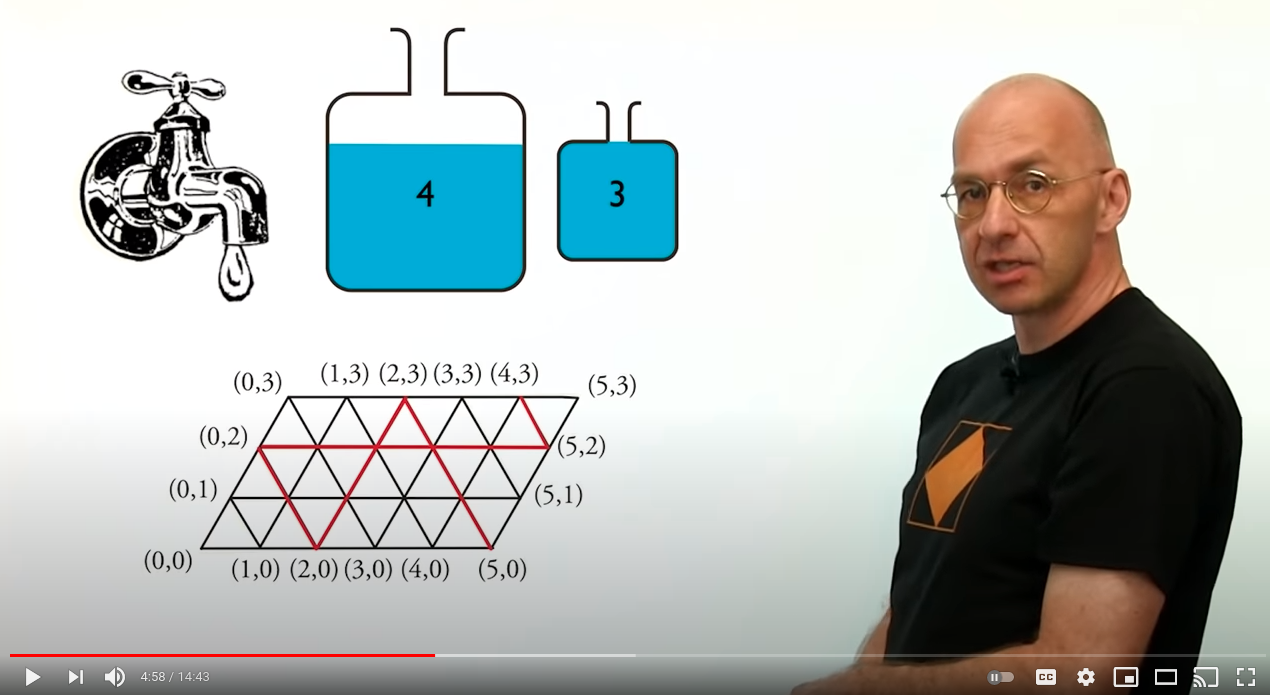
\includegraphics{mathologer.png}
		\caption{\href{https://www.youtube.com/watch?v=0Oef3MHYEC0}{Mathologer
		visual demonstration of this problem in action}}
	\end{figure}

	\vspace{1em}

	\begin{tabular}{|l|c|c|r|}
		\hline
		\thead{Step} & \thead{5 Gallon Jug} & \thead{3 Gallon jug}\\
		\hline
		Fill 5G jug from fountain & 5 & 0 \\
		Fill 3G jug from 5G jug & 2 & 3 \\
		Empty 3G jug & 2 & 0 \\
		Empty 5G jug into 3G jug & 0 & 2 \\
		Fill 5G jug from fountain & 5 & 2 \\
		Top up 3G jug from 5G jug & 4 & 3 \\
		\hline
		\multicolumn{3}{|c|}{\bfseries Weigh 5G jug} \\
		\hline
	\end{tabular}
	
	\vspace{1em}

	Now - given the relationship to B\'ezout's identity, can you find
	another solution which involves filling the 3G jug from the fountain?


\end{proof}

\begin{question}
What is the inverse of 10 modulo 17?
\end{question}

\begin{proof}[Answer]
	The multiplicative inverse of $k \pmod{n}$ in modular arithmetic is an integer which, when you
	multiply it by $k$, gives a result of $1 \pmod{n}$

	In other words, we need to find a number $m$ such that:
	\[ 10m + 17n = 1 \]

	We will use Euclid's algorithm to get the GCD of 10 and 17 (which is obviously 1):
	\begin{align*}
		17 &= 10 + 7 & 7 &= 17 - 10 \\
		10 &= 7 + 3  & 3 &= 10 - 7 \\
		7 &= 2 \times 3 + 1 & 1 &= 7 - 2 \times 3 \\
		&& 1 &= 7 - 2 \times (10 - 7) \\
		&& 1 &= 3 \times 7 - 2 \times 10 \\
		&& 1 &= 3 \times (17 - 10) - 2 \times 10 \\
		&& 1 &= 3 \times 17 - 5 \times 10 \\
	\end{align*}
	
	We have an identity, with a general term: 
	\[ 1  = (3 - 10k) \times 17 + (17k-5) \times 10 \]
	with the smallest positive multiple of 10 which works being $k=1$, $17-5 = 12$
	And it's easy to verify that $1 = 12\times10 - 7\times17$.
\end{proof}

\begin{question}Find a solution in integers to the Diophantine equation $61x + 23y = 1$\end{question}
\vspace*{\bigskipamount}

\begin{question}Find a natural number $k$ such that $(573k+4)/719$ is also a natural
number.\end{question}
\vspace*{\bigskipamount}

\begin{question}Find the smallest positive integer that ends in 2010, and is divisible by 2011.\end{question}
\vspace*{\bigskipamount}


\end{document}
